\documentclass{bioinfo}
\copyrightyear{2015} \pubyear{2015}

\access{ }
\appnotes{Manuscript Category}

\begin{document}
\firstpage{1}

\subtitle{Protein Classification}

\title[short Title]{Predicting Protein Origin from Sequence Data}
\author[Sample \textit{et~al}.]{Eric Hambro\,$^{\text{\sfb 1,}*}$}
\address{$^{\text{\sf 1}}$Department, Institution, City, Post Code, Country}

\corresp{$^\ast$To whom correspondence should be addressed.}

\history{ }

\editor{ }

\abstract{\textbf{Motivation:}  
Deriving protein function from sequence level data can provide.  Using features derived from the sequence and a random forests model was trained to classify protein sequences according to their location of use. Using a validation set of blah, an accuracy prediction accuracy of blah was reported, along with an F1 score of blah.\\
\textbf{Results:} Text  Text Text Text Text Text Text Text Text Text  Text Text Text Text Text
Text Text Text Text Text Text Text Text Text Text Text Text Text  Text Text Text Text Text Text\\
\textbf{Availability:} Text  Text Text Text Text Text Text Text Text Text  Text Text Text Text
Text Text Text Text Text Text Text Text Text Text Text Text Text Text  Text\\
\textbf{Contact:} \href{eric.hambro.17@ucl.ac.uk}{eric.hambro.17@ucl.ac.uk}
}

\maketitle

\section{Introduction}



Although sequence data of genes has proliferated since the advent of \textbf{technique}, the classification of protein function has lagged behind significantly.  \textbf{Statistic}. 
This is partly down to the fact that protein function is a complex labelling task, given the function of proteins may vary under different conditions.  
In cases where no homologues are present for a gene, knowing the subcellular location of the the protein gives indicator as to the proteins function. 
Furthermore discovering subcellular location has proven to be vital information in the research of new drugs and vaccinations. 
As such, automated means of predicting subcelular localization are utmost urgency in todays drug search enbironment.

Since as early as \textbf{blah}, machine learning has been used to predict automatically the subcellular localization of a protein, in an attempt to reduce the cost and time taken to process the proliferating protein sequences.   Traditional methods such as \textbf{experiment}, which were laborious and time intensive, have been replaced in parts by \text{papers}, which are able to make predictions at a high degree of confidence \textit{reference} with only sequence data.

Some these techniques include \textbf{machine learning technique}, which does a \textbf{xyz}, and \textbf{ml technique 2} which does \textbf{this}. 

In this particular experiment we are presented with a training data set \textit{X} proteins, each corresponding to one of four subcellular locations, and we train and evaluated a Random Forests classifier on these data, finally making predictions of locations for \textit{X} unknown proteins.  

Section 2 of this report contains a description of the method used, and Section 3 presents our results. A discussion of these results is then presented in Section 4, along with analyses of the features of the model, a comparison to another model, and our motivation in choosing this method.  Finally, I present a comparison with existing work in the field and further work that could be done, ending with a conclusion.
%Para 1: What is it & why is it important?
%Para 2: What are applications?
%Para 3: What is the history?

%In this analsysi we are presented with predicting 4 classes of locations: w, x, y, z. These are mutually exclusive categories, and our aim was to train a classifier to predict our things. 

%Section 2 of this report contains a description of the method, where section 3 presents the results. Section 4 presents a discussion of the results, breaking down the reasons for choosing the method, and providing analyses of the features, results and a comparison to another model. Finally, I present a comparison with existing work in the field and further work that could be done. 

 %is Often pro 
%Why is protein function hard to predict? What is protein location hard to predict? Why is it important?

\section{Method}

\subsection{Preprocessing}

Data was obtained from four files containing protein sequences in Fasta format. 
Each file contained proteins according to its type of subcellular localization: cytosolic, secreted, nuclear and mitochondrial. The number of proteins in each file is presented in Table \ref{Tab:RawData}. 
These data files contained no homologues, and therefore could be assimilated, shuffled and split into a training and validation set randomly. 

The data was then fed through a pipeline to extract a number of features from the sequence. Here the open source `BioPython` \textit{reference} module was used, which allowed us to augment sequence data with important characteristics of the amino acids, such as hydrophobicity or molecular weight. These features were : \
\begin{itemize}
\item{ Feature 1}
What is each one. a line or two.
\item{ Feature 2} 
\item{ Feature 1} 
\item{ Feature 1} 
\item{ Feature 1} 
\end{itemize}
. 


The numerical features were then concatenated to form a vector, and divided such that 30\% of the data formed a validation set, with the remainder forming a test set. An anlysis of the features themselves is present in section 4. 


\begin{table}[!t]
\processtable{Sample Data Set By Protein Class\label{Tab:RawData}} {\begin{tabular}{@{}llll@{}}\toprule Cytosolic &
Nucleic & Secreted & Mitochondrial\\\midrule
row4 & row4 & row4 & row4\\\botrule
\end{tabular}}{}
\end{table}

\subsection{Classifier Training}

A Random Forest Classifier was used in the training of the model, which was done with 70\% of the training data.  The classifier itself was implemented using the open source `scikit-learn` package, and was instantiated with the a \textbf{hyperparameters of X, Y, Z}. These hyperparameters were all chosen in advance using k-fold cross validation, and a grid search on hyper parameters.

\subsection{Cross Validation \& Hyperparameter Tuning}

In order to assess both the strength of model under certain hyperparameters, and the strength of the predictive power of certain features, a 5-fold cross validation score \textit{(what score?)} of the model was used, each time with a 70\%, 30\% train-validation split. In order to search the space of hyperparameters, a grid search was established, visible in plot \textit{plt the cross valid hyper param search}. 

\subsection{Ablation Study}

An ablation study was performed, by removing one feature at a time and testing the 5-fold cross validation score of the model in predicting these data. The results are presented \textit{fig xyz}

\subsection{Gradient Boosting Comparison}

The training set of features was then 


\section{Results}

\begin{figure}[h]
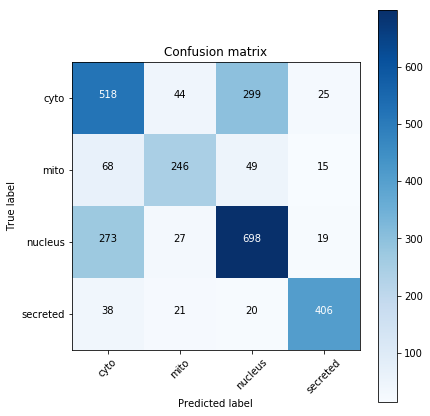
\includegraphics[width=8cm]{confusion}
\centering
\end{figure}

\begin{figure}[h]
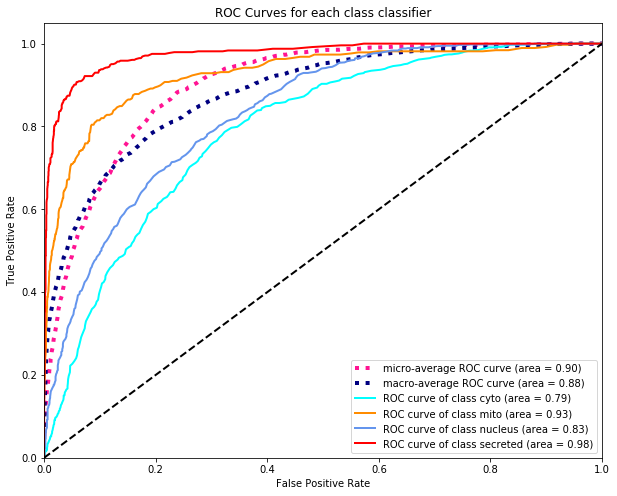
\includegraphics[width=8cm]{roc_curve}
\centering
\end{figure}


\begin{table}[!t]
\processtable{Predictions of Test Proteins\label{Tab:02}} {\begin{tabular}{@{}lll@{}}\toprule Protein ID  & Subcellular Location & Probabilty \\\midrule
row1 & row1 & row1 \\
row2 & row2 & row2 \\
row3 & row3 & row3 \\
row4 & row4 & row4 \\\botrule
\end{tabular}}{This is a footnote}
\end{table}



    - Results of accuracy
    - Confusion matrix
    - ablation study
    - results compared to xgboost


\newpage
yip
\newpage

Obtained data from X files, and mixed, shuffle and split into a train and validation split. Since the proteins are all non homolgoues, no need to arrange by family and could split anyway. 

Then took these files and processed them into feature vectors, using the bipython module. These extracted, x features from the sequence. 

Then trained a random forest classifier with X trees, and also tested a XGBboost classifier.

Cross validated grid search done to find best parameters for trees
Ablation study used to investigate salient features.

Trained a random forest with X trees. 

What did you do?
    - extract features
    - train -test split - homologies
    - cross validate
    - compared with a model (gradient boosting?)
    - ablation study



    - Results of accuracy
    - Confusion matrix
    - ablation study
    - results compared to xgboost
\section{Discussion}
   - Examine the features
   - Examine the ablation study
   - Examine comparison to XGBoost
   - Compare with existing literature and approaches



\section{Further Work}
    - suggestions: more data? better features/

\section{Conclusion}

\section{Theoretical Background}

What about ???
















\newpage
end of paper
\newpage

Text Text Text Text Text Text  Text Text Text Text Text Text Text
Text Text  Text Text Text Text Text Text. Figure~\ref{fig:01}
shows that the above method  Text Text Text Text  Text Text Text
Text Text Text  Text Text.  \citep{Bag01} wants to know about
{\ldots}{\ldots} text follows.
\begin{equation}
\sum \text{\it x}+ \text{\it y} =\text{\it Z}\label{eq:01}\vspace*{-10pt}
\end{equation}

%\enlargethispage{12pt}

\section{Approach}

Equation~(\ref{eq:01}) Text Text Text Text Text Text  Text Text
Text Text Text Text Text Text Text Text Text Text Text Text Text.
Figure~2\vphantom{\ref{fig:02}} shows that the above method  Text
Text Text Text  Text Text Text Text Text Text  Text Text.
\citealp{Boffelli03} might want to know about text text text text
.....


\begin{methods}
\section{Methods}

Text Text Text Text Text Text  Text Text Text Text Text Text Text
Text Text  Text Text Text Text Text Text.
Figure~2\vphantom{\ref{fig:02}} shows that the above method  Text
Text Text Text  Text Text Text Text Text Text  Text Text.
\citealp{Boffelli03} might want to know about  text text text text
Text Text Text Text Text Text Text Text Text Text Text Text Text
Text Text  Text Text Text Text Text Text.
Figure~2\vphantom{\ref{fig:02}} shows that the above method  Text
Text Text Text Text Text Text Text Text Text  Text Text.
\citealp{Boffelli03} might want to know about text text text text
Text Text Text Text Text Text  Text Text Text Text Text Text Text
Text Text Text Text Text Text Text Text.
Figure~2\vphantom{\ref{fig:02}} shows that the above method  Text
Text Text Text Text Text Text Text Text Text  Text Text.
\citealp{Boffelli03} might want to know about text text text
text\vspace*{1pt}

\begin{itemize}
\item for bulleted list, use itemize
\item for bulleted list, use itemize
\item for bulleted list, use itemize\vspace*{1pt}
\end{itemize}

Text Text Text Text Text Text  Text Text Text Text Text Text Text
Text Text  Text Text Text Text Text Text.
Figure~2\vphantom{\ref{fig:02}} shows that the above method  Text
Text Text Text  Text Text Text Text Text Text  Text Text.
\citealp{Boffelli03} might want to know about  text text text text
Text Text Text Text Text Text Text Text Text Text Text Text Text
Text Text Text Text Text Text Text Text.
Figure~2\vphantom{\ref{fig:02}} shows that the above method  Text
Text Text Text Text Text Text Text Text Text  Text Text.
\citealp{Boffelli03} might want to know about text text text text
Text Text Text Text Text Text  Text Text Text Text Text Text Text
Text Text Text Text Text Text Text Text.
Figure~2\vphantom{\ref{fig:02}} shows that the above method  Text
Text Text Text Text Text Text Text Text Text  Text Text.
\citealp{Boffelli03} might want to know about text text text text
Text Text Text Text Text Text  Text Text Text Text Text Text Text
Text Text Text Text Text Text Text Text.
Figure~2\vphantom{\ref{fig:02}} shows that the above method Text
Text Text Text Text Text Text Text Text Text Text Text.
\citealp{Boffelli03} might want to know about text text text text
Text Text Text Text Text Text  Text Text Text Text Text Text Text
Text Text Text Text Text Text Text Text.

Text Text Text Text Text Text  Text Text Text Text Text Text Text
Text Text  Text Text Text Text Text Text\vadjust{\newpage}.
Figure~2\vphantom{\ref{fig:02}} shows that the above method  Text
Text Text Text  Text Text Text Text Text Text  Text Text.
\citealp{Boffelli03} might want to know about text text text text
Text Text Text Text Text Text Text Text Text Text Text Text Text
Text Text Text Text Text Text Text Text.
Figure~2\vphantom{\ref{fig:02}} shows that the above method  Text
Text Text Text Text Text Text Text Text Text  Text Text.
\citealp{Boffelli03} might want to know about text text text text
Text Text Text Text Text Text  Text Text Text Text Text Text Text
Text Text Text Text Text Text Text Text.
Figure~2\vphantom{\ref{fig:02}} shows that the above method  Text
Text Text Text Text Text Text Text Text Text  Text Text.
\citealp{Boffelli03} might want to know about text text text text
Text Text Text Text Text Text  Text Text Text Text Text Text Text
Text Text Text Text Text Text Text Text.
Figure~2\vphantom{\ref{fig:02}} shows that the above method Text
Text Text Text Text Text Text Text Text Text Text Text.
\citealp{Boffelli03} might want to know about text text text text
Text Text Text Text Text Text  Text Text Text Text Text Text Text
Text Text Text Text Text Text Text Text.


Text Text Text Text Text Text  Text Text Text Text Text Text Text
Text Text  Text Text Text Text Text Text.
Figure~2\vphantom{\ref{fig:02}} shows that the above method  Text
Text Text Text  Text Text Text Text Text Text  Text Text.
\citealp{Boffelli03} might want to know about  text text text text
Text Text Text Text Text Text  Text Text Text Text Text Text Text
Text Text  Text Text Text Text Text Text.
Figure~2\vphantom{\ref{fig:02}} shows that the above method  Text
Text Text Text  Text Text Text Text Text Text  Text Text.
\citealp{Boffelli03} might want to know about  text text text text
Text Text Text Text Text Text Text Text Text Text Text Text Text
Text Text  Text Text Text Text Text Text.
Figure~2\vphantom{\ref{fig:02}} shows that the above method  Text
Text Text Text  Text Text Text Text Text Text  Text Text.
\citealp{Boffelli03} might want to know about  text text text text



Text Text Text Text Text Text  Text Text Text Text Text Text Text
Text Text  Text Text Text Text Text Text.
Figure~2\vphantom{\ref{fig:02}} shows that the above method  Text
Text Text Text  Text Text Text Text Text Text  Text Text.
\citealp{Boffelli03} might want to know about  text text text text
Text Text Text Text Text Text  Text Text Text Text Text Text Text
Text Text  Text Text Text Text Text Text.
Figure~2\vphantom{\ref{fig:02}} shows that the above method  Text
Text Text Text  Text Text Text Text Text Text  Text Text.
\citealp{Boffelli03} might want to know about  text text text text
Text Text Text Text Text Text Text Text Text Text Text Text Text
Text Text  Text Text Text Text Text Text.

\subsection{This is subheading}

Text Text Text Text Text Text  Text Text Text Text Text Text Text
Text Text  Text Text Text Text Text Text.
Figure~2\vphantom{\ref{fig:02}} shows that the above method  Text
Text Text Text  Text Text Text Text Text Text  Text Text.
\citealp{Boffelli03} might want to know about  text text text text
Text Text Text Text Text Text  Text Text Text Text Text Text Text
Text Text  Text Text Text Text Text Text.
Figure~2\vphantom{\ref{fig:02}} shows that the above method  Text
Text Text Text Text Text Text Text Text Text  Text Text.
\citealp{Boffelli03} might want to know about  text text text text
Text Text Text Text Text Text Text Text Text Text Text Text Text
Text Text  Text Text Text Text Text Text.
Figure~2\vphantom{\ref{fig:02}} shows that the above method  Text
Text Text Text Text Text Text Text Text Text  Text Text.
\citealp{Boffelli03} might want to know about  text text text
text. Text Text Text Text Text Text  Text Text Text Text Text Text
Text Text Text  Text Text Text Text Text Text.
Figure~2\vphantom{\ref{fig:02}} shows that the above method  Text
Text Text Text Text Text Text Text Text Text  Text Text.
\citealp{Boffelli03} might want to know about  text text text text
Text Text Text Text Text Text Text Text Text Text Text Text Text
Text Text  Text Text Text Text Text Text.
Figure~2\vphantom{\ref{fig:02}} shows that the above method  Text
Text Text Text Text Text Text Text Text Text  Text Text.
\citealp{Boffelli03} might want to know about  text text text text
Text Text Text Text Text Text  Text Text Text Text Text Text Text
Text Text  Text Text Text Text Text Text.
Figure~2\vphantom{\ref{fig:02}} shows that the above method  Text
Text Text Text Text Text Text Text Text Text  Text Text.
\citealp{Boffelli03} might want to know about  text text text text
Text Text Text Text Text Text Text Text Text Text Text Text Text
Text Text  Text Text Text Text Text Text.
Figure~2\vphantom{\ref{fig:02}} shows that the above method  Text
Text Text Text Text Text Text Text Text Text  Text Text.
\citealp{Boffelli03} might want to know about  text text text text
Text Text Text Text Text Text  Text Text Text Text Text Text Text
Text Text  Text Text Text Text Text Text.


\subsubsection{This is subsubheading}

Text Text Text Text Text Text  Text Text Text Text Text Text Text
Text Text  Text Text Text Text Text Text.
Figure~2\vphantom{\ref{fig:02}} shows that the above method  Text
Text Text Text  Text Text Text Text Text Text  Text Text.
\citealp{Boffelli03} might want to know about  text text text text
Text Text Text Text Text Text  Text Text Text Text Text Text Text
Text Text  Text Text Text Text Text Text.
Figure~2\vphantom{\ref{fig:02}} shows that the above method  Text
Text Text Text  Text Text Text Text Text Text  Text Text.
\citealp{Boffelli03} might want to know about  text text text text
Text Text Text Text Text Text Text Text Text Text Text Text Text
Text Text  Text Text Text Text Text Text.
Figure~2\vphantom{\ref{fig:02}} shows that the above method  Text
Text Text Text  Text Text Text Text Text Text  Text Text.
\citealp{Boffelli03} might want to know about  text text text text



Text Text Text Text Text Text  Text Text Text Text Text Text Text
Text Text  Text Text Text Text Text Text.
Figure~2\vphantom{\ref{fig:02}} shows that the above method  Text
Text Text Text  Text Text Text Text Text Text  Text Text.
\citealp{Boffelli03} might want to know about  text text text text
Text Text Text Text Text Text  Text Text Text Text Text Text Text
Text Text  Text Text Text Text Text Text.
Figure~2\vphantom{\ref{fig:02}} shows that the above method  Text
Text Text Text  Text Text Text Text Text Text  Text Text.
\citealp{Boffelli03} might want to know about  text text text text
Text Text Text Text Text Text Text Text Text Text Text Text Text
Text Text  Text Text Text Text Text Text.
Figure~2\vphantom{\ref{fig:02}} shows that the above method  Text
Text Text Text  Text Text Text Text Text Text  Text Text.
\citealp{Boffelli03} might want to know about  text text\break
text text


Text Text Text Text Text Text  Text Text Text Text Text Text Text
Text Text  Text Text Text Text Text Text.
Figure~2\vphantom{\ref{fig:02}} shows that the above method  Text
Text Text Text  Text Text Text Text Text Text  Text Text.
\citealp{Boffelli03} might want to know about  text text text text
Text Text Text Text Text Text  Text Text Text Text Text Text Text
Text Text  Text Text Text Text Text Text.
Figure~2\vphantom{\ref{fig:02}} shows that the above method  Text
Text Text Text  Text Text Text Text Text Text  Text Text.
\citealp{Boffelli03} might want to know about  text text text text
Text Text Text Text Text Text Text Text Text Text Text Text Text
Text Text  Text Text Text Text Text Text.
Figure~2\vphantom{\ref{fig:02}} shows that the above method  Text
Text Text Text  Text Text Text Text Text Text  Text Text.
\citealp{Boffelli03} might want to know about  text text text
textText Text Text Text Text Text  Text Text Text Text Text Text
Text Text Text  Text Text Text Text Text Text.
Figure~2\vphantom{\ref{fig:02}} shows that the above method  Text
Text Text Text  Text Text Text Text Text Text  Text Text.
\citealp{Boffelli03} might want to know about  text text text text
Text Text Text Text Text Text Text Text Text Text Text Text Text
Text Text  Text Text Text Text Text Text.
Figure~2\vphantom{\ref{fig:02}} shows that the above method  Text
Text Text Text  Text Text Text Text Text Text  Text Text.
\citealp{Boffelli03} might want to know about  text text text text
Text Text Text Text Text Text  Text Text Text Text Text Text Text
Text Text  Text Text Text Text Text Text.
Figure~2\vphantom{\ref{fig:02}} shows that the above method  Text
Text Text Text  Text Text Text Text Text Text  Text Text.
\citealp{Boffelli03} might want to know about  text text text text
Text Text Text Text Text Text Text Text Text Text Text Text Text
Text Text  Text Text Text Text Text Text.
Figure~2\vphantom{\ref{fig:02}} shows that the above method  Text
Text Text Text  Text Text Text Text Text Text  Text Text.
\citealp{Boffelli03} might want to know about  text text text text
Text Text Text Text Text Text  Text Text Text Text Text Text Text
Text Text  Text Text Text Text Text Text.

\enlargethispage{6pt}


Text Text Text Text Text Text  Text Text Text Text Text Text Text
Text Text  Text Text Text Text Text Text.
Figure~2\vphantom{\ref{fig:02}} shows that the above method  Text
Text Text Text  Text Text Text Text Text Text  Text Text.
\citealp{Boffelli03} might want to know about  text text text text
Text Text Text Text Text Text  Text Text Text Text Text Text Text
Text Text  Text Text Text Text Text Text.
Figure~2\vphantom{\ref{fig:02}} shows that the above method  Text
Text Text Text  Text Text Text Text Text Text  Text Text.
\citealp{Boffelli03} might want to know about  text text text text
Text Text Text Text Text Text Text Text Text Text Text Text Text
Text Text  Text Text Text Text Text Text.
Figure~2\vphantom{\ref{fig:02}} shows that the above method  Text
Text Text Text  Text Text Text Text Text Text  Text Text.
\citealp{Boffelli03} might want to know about  text text text text



Text Text Text Text Text Text  Text Text Text Text Text Text Text
Text Text  Text Text Text Text Text Text.
Figure~2\vphantom{\ref{fig:02}} shows that the above method  Text
Text Text Text  Text Text Text Text Text Text  Text Text.
\citealp{Boffelli03} might want to know about  text text text text
Text Text Text Text Text Text  Text Text Text Text Text Text Text
Text Text  Text Text Text Text Text Text.
Figure~2\vphantom{\ref{fig:02}} shows that the above method  Text
Text Text Text  Text Text Text Text Text Text  Text Text.
\citealp{Boffelli03} might want to know about  text text text text
Text Text Text Text Text Text Text Text Text Text Text Text Text
Text Text  Text Text Text Text Text Text.
Figure~2\vphantom{\ref{fig:02}} shows that the above method  Text
Text Text Text  Text Text Text Text Text Text  Text Text.
\citealp{Boffelli03} might want to know about  text text text text


Text Text Text Text Text Text  Text Text Text Text Text Text Text
Text Text  Text Text Text Text Text Text.
Figure~2\vphantom{\ref{fig:02}} shows that the above method  Text
Text Text Text  Text Text Text Text Text Text  Text Text.
\citealp{Boffelli03} might want to know about  text text text text
Text Text Text Text Text Text  Text Text Text Text Text Text Text
Text Text  Text Text Text Text Text Text.
Figure~2\vphantom{\ref{fig:02}} shows that the above method  Text
Text Text Text  Text Text Text Text Text Text  Text Text.
\citealp{Boffelli03} might want to know about  text text text text
Text Text Text Text Text Text Text Text Text Text Text Text Text
Text Text  Text Text Text Text Text Text.
Figure~2\vphantom{\ref{fig:02}} shows that the above method  Text
Text Text Text  Text Text Text Text Text Text  Text Text.
\citealp{Boffelli03} might want to know about  text text text text

Text Text Text Text Text Text  Text Text Text Text Text Text Text
Text Text  Text Text Text Text Text Text.
Figure~2\vphantom{\ref{fig:02}} shows that the above method  Text
Text Text Text  Text Text Text Text Text Text  Text Text.
\citealp{Boffelli03} might want to know about  text text text text
Text Text Text Text Text Text  Text Text Text Text Text Text Text
Text Text  Text Text Text Text Text Text.
Figure~2\vphantom{\ref{fig:02}} shows that the above method  Text
Text Text Text  Text Text Text Text Text Text  Text Text.
\citealp{Boffelli03} might want to know about  text text text text
Text Text Text Text Text Text Text Text Text Text Text Text Text
Text Text  Text Text Text Text Text Text.
Figure~2\vphantom{\ref{fig:02}} shows that the above method  Text
Text Text Text  Text Text Text Text Text Text  Text Text.
\citealp{Boffelli03} might want to know about  text text text text
Text Text Text Text Text Text  Text Text Text Text Text Text Text
Text Text  Text Text Text Text Text Text.
Figure~2\vphantom{\ref{fig:02}} shows that the above method  Text
Text Text Text  Text Text Text Text Text Text  Text Text.
\citealp{Boffelli03} might want to know about  text text text text
Text Text Text Text Text Text Text Text Text Text Text Text Text
Text Text  Text Text Text Text Text Text.


Text Text Text Text Text Text  Text Text Text Text Text Text Text
Text Text  Text Text Text Text Text Text.
Figure~2\vphantom{\ref{fig:02}} shows that the above method  Text
Text Text Text  Text Text Text Text Text Text  Text Text.
\citealp{Boffelli03} might want to know about  text text text text
Text Text Text Text Text Text  Text Text Text Text Text Text Text
Text Text  Text Text Text Text Text Text.
Figure~2\vphantom{\ref{fig:02}} shows that the above method  Text
Text Text Text  Text Text Text Text Text Text  Text Text.
\citealp{Boffelli03} might want to know about  text text text text
Text Text Text Text Text Text Text Text Text Text Text Text Text
Text Text  Text Text Text Text Text Text.
Figure~2\vphantom{\ref{fig:02}} shows that the above method  Text
Text Text Text  Text Text Text Text Text Text  Text Text.
\citealp{Boffelli03} might want to know about  text text text text

\begin{table}[!t]
\processtable{This is table caption\label{Tab:01}} {\begin{tabular}{@{}llll@{}}\toprule head1 &
head2 & head3 & head4\\\midrule
row1 & row1 & row1 & row1\\
row2 & row2 & row2 & row2\\
row3 & row3 & row3 & row3\\
row4 & row4 & row4 & row4\\\botrule
\end{tabular}}{This is a footnote}
\end{table}

\end{methods}

\begin{figure}[!tpb]%figure1
\fboxsep=0pt\colorbox{gray}{\begin{minipage}[t]{235pt} \vbox to 100pt{\vfill\hbox to
235pt{\hfill\fontsize{24pt}{24pt}\selectfont FPO\hfill}\vfill}
\end{minipage}}
%\centerline{\includegraphics{fig01.eps}}
\caption{Caption, caption.}\label{fig:01}
\end{figure}

%\begin{figure}[!tpb]%figure2
%%\centerline{\includegraphics{fig02.eps}}
%\caption{Caption, caption.}\label{fig:02}
%\end{figure}

Text Text Text Text Text Text  Text Text Text Text Text Text Text
Text Text  Text Text Text Text Text Text.
Figure~2\vphantom{\ref{fig:02}} shows that the above method  Text
Text Text Text  Text Text Text Text Text Text  Text Text.
\citealp{Boffelli03} might want to know about  text text text text
Text Text Text Text Text Text  Text Text Text Text Text Text Text
Text Text  Text Text Text Text Text Text.
Figure~2\vphantom{\ref{fig:02}} shows that the above method  Text
Text Text Text  Text Text Text Text Text Text  Text Text.
\citealp{Boffelli03} might want to know about  text text text text
Text Text Text Text Text Text Text Text Text Text Text Text Text
Text Text  Text Text Text Text Text Text.
Figure~2\vphantom{\ref{fig:02}} shows that the above method  Text
Text Text Text  Text Text Text Text Text Text  Text Text.
\citealp{Boffelli03} might want to know about  text text text text


\subsection{Test1}

Text Text Text Text Text Text  Text Text Text Text Text Text Text
Text Text  Text Text Text Text Text Text.
Figure~2\vphantom{\ref{fig:02}} shows that the above method  Text
Text Text Text  Text Text Text Text Text Text  Text Text.
\citealp{Boffelli03} might want to know about  text text text text
Text Text Text Text Text Text  Text Text Text Text Text Text Text
Text Text  Text Text Text Text Text Text.
Figure~2\vphantom{\ref{fig:02}} shows that the above method  Text
Text Text Text  Text Text Text Text Text Text  Text Text.
\citealp{Boffelli03} might want to know about  text text text text
Text Text Text Text Text Text Text Text Text Text Text Text Text
Text Text  Text Text Text Text Text Text.
Figure~2\vphantom{\ref{fig:02}} shows that the above method  Text
Text Text Text  Text Text Text Text Text Text  Text Text.
\citealp{Boffelli03} might want to know about  text text text text





\section{Discussion}

Text Text Text Text Text Text  Text Text Text Text Text Text Text
Text Text  Text Text Text Text Text Text.
Figure~2\vphantom{\ref{fig:02}} shows that the above method  Text
Text Text Text  Text Text Text Text Text Text  Text Text.
\citealp{Boffelli03} might want to know about  text text text text
Text Text Text Text Text Text  Text Text Text Text Text Text Text
Text Text  Text Text Text Text Text Text.
Figure~2\vphantom{\ref{fig:02}} shows that the above method  Text
Text Text Text  Text Text Text Text Text Text  Text Text.
\citealp{Boffelli03} might want to know about  text text text text
Text Text Text Text Text Text Text Text Text Text.




Table~\ref{Tab:01} shows that Text Text Text Text Text  Text Text
Text Text Text Text. Figure~2\vphantom{\ref{fig:02}} shows that
the above method Text Text. Text Text Text  Text Text Text Text
Text Text. Figure~2\vphantom{\ref{fig:02}} shows that the above
method Text Text. Text Text Text  Text Text Text Text Text Text.
Figure~2\vphantom{\ref{fig:02}} shows that the above method Text
Text.









%%%%%%%%%%%%%%%%%%%%%%%%%%%%%%%%%%%%%%%%%%%%%%%%%%%%%%%%%%%%%%%%%%%%%%%%%%%%%%%%%%%%%
%
%     please remove the " % " symbol from \centerline{\includegraphics{fig01.eps}}
%     as it may ignore the figures.
%
%%%%%%%%%%%%%%%%%%%%%%%%%%%%%%%%%%%%%%%%%%%%%%%%%%%%%%%%%%%%%%%%%%%%%%%%%%%%%%%%%%%%%%






\section{Conclusion}

(Table~\ref{Tab:01}) Text Text Text Text Text Text  Text Text Text
Text Text Text Text Text Text  Text Text Text Text Text Text.
Figure~2\vphantom{\ref{fig:02}} shows that the above method  Text
Text Text Text  Text Text Text Text Text Text  Text Text.
\citealp{Boffelli03} might want to know about  text text text text
Text Text Text Text Text Text  Text Text Text Text Text Text Text
Text Text  Text Text Text Text Text Text.
Figure~2\vphantom{\ref{fig:02}} shows that the above method  Text
Text Text Text  Text Text Text Text Text Text  Text Text.
\citealp{Boffelli03} might want to know about  text text text text
Text Text Text Text Text Text Text Text Text Text Text Text Text
Text Text  Text Text Text Text Text Text.
Figure~2\vphantom{\ref{fig:02}} shows that the above method  Text
Text Text Text  Text Text Text Text Text Text  Text Text.



Text Text Text Text Text Text  Text Text Text Text Text Text Text
Text Text  Text Text Text Text Text Text.
Figure~2\vphantom{\ref{fig:02}} shows that the above method  Text
Text Text Text  Text Text Text Text Text Text  Text Text.
\citealp{Boffelli03} might want to know about  text text text text

\begin{enumerate}
\item this is item, use enumerate
\item this is item, use enumerate
\item this is item, use enumerate
\end{enumerate}

Text Text Text Text Text Text Text Text Text Text Text Text Text
Text Text Text Text Text Text Text Text.
Figure~2\vphantom{\ref{fig:02}} shows\vadjust{\pagebreak} that the
above method  Text Text Text Text Text Text Text Text Text Text
Text Text.  \citealp{Boffelli03} might want to know about text
text text text Text Text Text Text Text Text  Text Text Text Text
Text Text Text Text Text Text Text Text Text Text Text.
Figure~2\vphantom{\ref{fig:02}} shows that the above method  Text
Text Text Text Text Text Text Text Text Text  Text Text.
\citealp{Boffelli03} might want to know about text text text text
Text Text Text Text Text Text  Text Text Text Text Text Text Text
Text Text Text Text Text Text Text\break Text.


Text Text Text Text Text Text  Text Text Text Text Text Text Text
Text Text  Text Text Text Text Text Text.
Figure~2\vphantom{\ref{fig:02}} shows that the above method  Text
Text Text Text\vspace*{-10pt}


\section*{Acknowledgements}

Text Text Text Text Text Text  Text Text.  \citealp{Boffelli03} might want to know about  text
text text text\vspace*{-12pt}

\section*{Funding}

This work has been supported by the... Text Text  Text Text.\vspace*{-12pt}

%\bibliographystyle{natbib}
%\bibliographystyle{achemnat}
%\bibliographystyle{plainnat}
%\bibliographystyle{abbrv}
%\bibliographystyle{bioinformatics}
%
%\bibliographystyle{plain}
%
%\bibliography{Document}


\begin{thebibliography}{}

\bibitem[Bofelli {\it et~al}., 2000]{Boffelli03}
Bofelli,F., Name2, Name3 (2003) Article title, {\it Journal Name}, {\bf 199}, 133-154.

\bibitem[Bag {\it et~al}., 2001]{Bag01}
Bag,M., Name2, Name3 (2001) Article title, {\it Journal Name}, {\bf 99}, 33-54.

\bibitem[Yoo \textit{et~al}., 2003]{Yoo03}
Yoo,M.S. \textit{et~al}. (2003) Oxidative stress regulated genes
in nigral dopaminergic neurnol cell: correlation with the known
pathology in Parkinson's disease. \textit{Brain Res. Mol. Brain
Res.}, \textbf{110}(Suppl. 1), 76--84.

\bibitem[Lehmann, 1986]{Leh86}
Lehmann,E.L. (1986) Chapter title. \textit{Book Title}. Vol.~1, 2nd edn. Springer-Verlag, New York.

\bibitem[Crenshaw and Jones, 2003]{Cre03}
Crenshaw, B.,III, and Jones, W.B.,Jr (2003) The future of clinical
cancer management: one tumor, one chip. \textit{Bioinformatics},
doi:10.1093/bioinformatics/btn000.

\bibitem[Auhtor \textit{et~al}. (2000)]{Aut00}
Auhtor,A.B. \textit{et~al}. (2000) Chapter title. In Smith, A.C.
(ed.), \textit{Book Title}, 2nd edn. Publisher, Location, Vol. 1, pp.
???--???.

\bibitem[Bardet, 1920]{Bar20}
Bardet, G. (1920) Sur un syndrome d'obesite infantile avec
polydactylie et retinite pigmentaire (contribution a l'etude des
formes cliniques de l'obesite hypophysaire). PhD Thesis, name of
institution, Paris, France.

\end{thebibliography}
\end{document}
